\documentclass[a4paper,12pt]{extarticle}

%% Language and font encodings
\usepackage[english]{babel}
\usepackage[utf8x]{inputenc}
\usepackage[T1]{fontenc}

%% Sets page size and margins
\usepackage[a4paper,top=3cm,bottom=2.5cm,left=3.5cm,right=3.5cm,marginparwidth=2cm]{geometry}

%% Useful packages
\usepackage{amsmath}
\usepackage{graphicx}
\usepackage[colorinlistoftodos]{todonotes}
\usepackage[colorlinks=true, allcolors=blue]{hyperref}

\title{Requirement Specification and Functional Design for Public Distribution System in India}
\author{Pratyush Maini, 
\\
Department of Computer Science and Engineering, 
\\
Indian Institute of Technology Delhi}

\begin{document}
\maketitle

\begin{abstract}
The Public Distribution System (\textbf{PDS}) is an important part of \textbf{food security} policy of a welfare state like India. A supposedly seeming simple task of distributing food grains to the poor and needy has many challenges. Hastily deployed technocratic designs among the under-privileged with poorly analysed and incomplete use cases and without adequate understanding of the social and cultural context can cause distress. This paper aims to analyse the \textbf{requirements} for an effective PDS system, and then goes on to describe a\textbf{ Functional design} for the same. I will highlight and focus on the functional requirements and  design changes for the \textbf{transaction process at the Fair Price Shops (FPS)}, especially focusing on a design that removes bindings of users with particular FPSs.
\end{abstract}

\section{Introduction}

The Indian democracy boasts of having the largest work force in the world. As a result, it is imperative to ensure the \textbf{health and nutrition }of your most valuable resource. The PDS is an important cog that ensures availability of food grains to the public at \textbf{affordable} prices, enhances the food security for the poor, specially in a country where a huge part of this workforce is struggling to make their ends meet.

The PDS has grown over the years, and currently has a network of over \textbf{5 lakh Fair Price Shops} (FPS) and is the largest distribution network of its type in the world. While both the union and the central goverment are responsible for the procurement, storage, transportation and bulk allocation of food grains to respective godowns, the state is solely responsible for managing the functioning of the FPSs.

At present the government has pressed towards making \textbf{AADHAR Based Biometric Authentication (ABBA)} mandatory to procure food grains. The system has been heavily critiqued for its inability to be a reliable source of authentication. It has been marred by problems such as biometric failure, lack of internet connectivity etc.

Through this paper, I present a design to model the system of Fair Price Shops in India, that is usable by the commoners and at the same time secure from unwanted sources of corruption. The model builds on the\textbf{ need to automate} the functioning of Fair Price Shops, as also proposed by the government. However, my path to achieving the same goal is different.


\subsection{Role of Aadhaar in Public Distribution System}
As per the policy laid by the Government of India, commodities shall be sold to beneficiaries after biometrics authentication with Aadhaar Server. Aadhaar Authentication API 1.6 is used for the authentication. 

1.	Aadhaar Seeding: The FPS Automation application shall have a provision of Aadhaar seeding. 

2.	Deferred authentication: In case of network un-availability, deferred authentication can be performed. Re-trial for Deferred authentication of fingerprints shall be carried out within next 24 hours as per UIDAI policy. Refer section 6.2 for more details on how deferred authentication shall be achieved. 

3.	IRIS authentication or OTP: If fingerprints authentication fails, then IRIS authentication will be done. In case of IRIS authentication failure, OTP shall be used. These options will be applicable if the state opts for the same.

\subsection{The Necessity of AADHAR}
As far as corruption in the PDS is concerned, Tamil Nadu has been running a clean system without UID. Intelligent applications of simpler technology (for example, computerisation, SMS alerts etc.), along with other
reforms, have contributed to the turnaround of the PDS in Chhattisgarh and Odisha. In these states estimated leakages of PDS grain have come down from around 50\% in both states, to 10\% and 20\% respectively (between 2004-2005 and 2010-2011).
These figures and precedences point to us that while digitisation is the need of the hour, it might not be necessary to enter the room through the door labeled AADHAR.

\section{Challenges with the Present System}

\subsection{Quality Fraud}
The process of transfer of grains from farmers to godowns and from godowns to Fair Price Shops is largely unregulated. The same leads plenty of opportunities for middlemen to replace the grain with stones or other low quality grains. The procured grains are then sold in the open market at higher prices, without the restrictions of government subsidy.

\subsection{Leakages and Quantity Fraud}
Large scale pilferages resulting from diversion and leakages of food grains meant for the poor populace of this country is the bane of the Targeted Public Distribution System. Manual processes related to PDS operations and specifically FPS sale are manual in nature which lead to a lot of diversions as it is not possible to probe whether actual sale happened at FPS or not. The key to make the distribution system uninfected is to ensure the fair Last Mile Delivery of essential commodities.



\subsection{Monopoly of Fair Price Shop Owners}
\begin{figure}
\centering
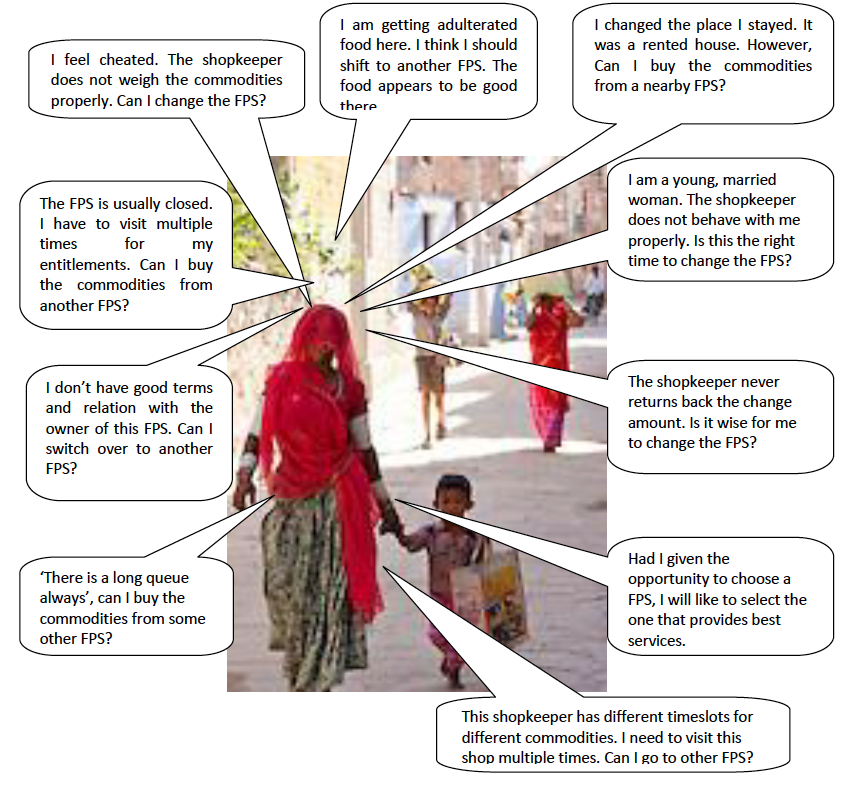
\includegraphics[width=0.9\textwidth]{CORE.png}
\caption{\label{fig:CORE}An illustration from the CORE PDS case study.}
\end{figure}
There are many concerns that arise among the beneficiaries owing to restriction of the choice of Fair Price Shop that they can go to.

\begin{itemize}
\item  The FPS is usually not open during the scheduled timings especially in the last two weeks of the month necessitating the beneficiaries multiple visits to the shop. This is a troublesome situation especially for those who could not avail the facilities in the first two weeks.
\item  Because of the prevalent monopoly, the FPS dukandar declares “no stock” - at times, even when the FPS has sufficient stocks - forcing the beneficiary multiple visits.
\item  The sales person does not accord due respect to the beneficiary or sometimes misbehaves. This is mainly because, in most of the FPSs, the customer is a women and sales person is generally a man. The literacy level is low.
\item  The sales person charges more than actual amount.
\item  Deliberate under weighing of the commodities by sales person.
\item  Adulteration of commodities by the dukandar before being issued to beneficiaries.
\item  It is also seen that, many a times, the beneficiaries may need to spend more than 4 to 5 hours in a queue to avail the benefits.
\end{itemize}
Traditionally, a beneficiary (family holding a valid ration card) is assigned to only one Fair Price Shop (FPS) to get their ‘food grain/s and kerosene’ entitlements at subsidized prices. The prices are usually decided by the state and/or central government. This creates a forced monopoly of the seller or the dukandar (the fair price shopkeeper). At times, it is seen that this monopoly deteriorates the service level and the beneficiaries are deprived of their rights.



\subsection{Exclusion From AADHAR roles}
The PDS system functions on a per capita term in the Below Poverty Household and per family term in the Antyodaya houses. 
The concern becomes of great importance in cases of old people or young children who are unable to get themselves on the AADHAR roles, either due to inability to travel from one place to other or due to lack of proper identification / enrollment opportunities.

\subsection{Failure of Biometrics (ABBA)}
The use of biometrics for identification purposes is still a growing technology and it often shows up false positives or negatives. As a result the problem of failure of biometrics is pretty genuine. 
This problem rose to the news headlines when 5 people died in a village in Jharkhand in 2017 due to inability to get their ration supplies.
The official records show a near 60\% success rate of transactions.

\subsection{Lack of Internet Connectivity}
Any policy decision being taken in the Indian context can not be taken aloof from the reality of lack of internet access. The requirement of authentication from the server for biometrics as a result is a very daunting task. Even though specific measures have been taken by the government to ensure connectivity at the fair price shops, the ambition of a well connected network of PDS, stays far from reality.


\subsection{Other Constraints}
\begin{itemize}
\item \textbf{Reflection in PDS cycle of new, modified or deleted Ration Cards}: The modifications in Ration Card will be reflected in next month allocation and distribution cycle. This is not done in real time to avoid inconsistency at any level of Public Distribution cycle. 
\item \textbf{Minimum battery for UIDAI authentication}: Minimum battery requirement for UIDAI authentication is 15-25%.
\item \textbf{Weighing machine}: If not calibrated in regular intervals, weighing machine gives undue advantage to Fair Price Shop owners. Hence binding of weighing machine with handheld device is not advisable.
\end{itemize}

\section{Building upon Success Stories}
\subsection{Tamil Nadu}

Tamil Nadu has always run a \textbf{universal PDS}. Implementation of NFSA in Thanjavur has been done via \textbf{QR-coded smart cards}. 

Smart card readers (a variant of the POS machine) maintain a\textbf{ digital trail} of all transactions (important from the point of view of bringing transparency to ensure accountability).

The smart readers, however, dispense with the requirement of reliable internet connectivity (they can work in offline mode, with transaction records being uploaded as and when connectivity is available). Since no biometric authentication is involved, it also does away with another vulnerability of Jharkhand’s ABBA system.

\subsection{Chhattisgarh}
The most notable changes were accompanied by Chhattisgarh’s \textbf{CORE PDS }experiment that began in 2012. They used smart cards with an embedded memory chip. Each transaction was recorded on the chip and made available online through the POS machine.

These two measures \textbf{de-privatising ration shops} and \textbf{doorstep delivery} of ration to Fair Price Shops were accompanied by \textbf{rigorous monitoring, often involving creative uses of technology.} For instance, a system of\textbf{ “SMS alerts” }was launched to inform interested citizens (more than 15,000 have already registered) of grain movements, and all \textbf{records pertaining to supplies, sales, timelines, etc.} were computerised. This involved much learning-bydoing. For instance, at one point the state government tried distributing pre-packed sacks of 35kg to prevent cheating, but the practice had to be discontinued as it was found that these sacks were being tampered with too. Therefore, in recent months, a move towards\textbf{ electronic weighing machines }has been initiated. Perhaps the most important step was \textbf{improved grievance redressal}, based, for instance, on active helplines. 



\section{Functional Requirements}

\subsection{Easy to use and Hassle Free}
The first and most important consideration for any technology to be implemented in a country like India is that it must be \textbf{usable by the poor and largely illiterate and uneducated population} of India. Specifically, the PDS system aims to target those sections of the society that have lie below the poverty line. Indeed, correlations between poverty and lack of education have been drawn for long in the Indian democracy. 

Therefore, this must be an important feature of our PDS system. We can not be expecting our users to change their lifestyle habits. Rather, it is important to make a system that aligns with the lifestyle of the users. Considering that a large proportion of our users are illiterate, we also need to enforce measures that does not alienate them from the use of the technology.

The second consideration of being\textbf{ hassle free }is also important, since we do not want the task of procuring grains from the Fair Price Shop to become a marathon task in itself. Even though there is no denial of the fact that there needs to be proper authentication of the customers, but at the same time we must remain minimalistic in our approach. The new system \textbf{must not} \textbf{disincentive} users from going to the FPS to procure grains.

\subsection{Distributed FPS Availability}

Even though de-allocation of FPSs can cause grain quantity mismatch in the short while, we see it gaining equlibrium in a span of weeks to restore the right quantity through appropriate measures on closing balance.
The Figure 1 is a beautiful illustration of the need for such a measure. 

The moment we deallocate a given user from a fixed shop, we gain a lot of benefits:
\begin{enumerate}
\item  \textbf{Competition among FPS owners}: Now that their potential customers are no longer fixed, the shopkeepers have much more incentive to look into the quality of service they provide. They will not only have to get rid of any corrupt and malpractices that they had been following, but will also work towards improving customer service.
\item \textbf{Freedom to the Customer:} The users will have much more freedom to choose between various shops in their district. Note that this allocation still can not happen outside the district as the rules for allocation vary from district to district.
\item \textbf{Users get Voice:} The most important part about the functioning of any democracy is that it mist give voice to the common man. Giving users this choice makes them feel a sense of belonging and responsibility towards the system. This is an important step towards an inclusive democracy.
\end{enumerate}


\subsection{Application and Data Security}

\begin{enumerate}
\item \textbf{Device Binding}: FPS device numbers are added / deleted from PDS server only. Only registered FPS MAC Ids can function within PDS system.
\item \textbf{Application Encryption}: The release version of the application shall be encrypted by algorithm and key given by NIC before deployment in the devices. In case the transactional data/application is tried to be tampered, the application shall get corrupt.
\item \textbf{Data Encryption}: The release version of the application shall be encrypted by algorithm and key given by NIC before deployment in the devices. In case the transactional data/application is tried to be tampered, the application shall get corrupt.
\item \textbf{Audit Trials}: The result codes of transactions are logged for each FPS, indicating the reason of success or failure. It will also be logged whether the device has a SIM inserted or not along with the timestamp and duration thereof.
\item \textbf{Route Officer Binding}: Only registered Route officers (or Distribution Officer/Inspector) can deliver commodity to FPS owner within PDS system.
\end{enumerate}

\subsection{Grievance Redressal Mechanism}
At the end of each functional design, we rely on the credibility of the people in the supply chain. However, it is the natural human instinct to gain greater profits from the resources at hand. People often look for ways to cheat the system when the incentives to obey the same are less.

It is imperative to ensure that the new PDS system has an active grievance redressal mechanism that curbs middlemen and FPS owners from indulging into any unwanted practices.

\subsection{Working in the Offline Mode}
The use of the PDS must not be constrained by the availability of internet connectivity which can be erratic and unachievable in many rural parts of the country. Any policy decision being taken in the Indian context can not be taken aloof from the reality of lack of internet access.  Even though specific measures have been taken by the government to ensure connectivity at the fair price shops, the ambition of a well connected network of PDS, stays far from reality.



\section{Functional Design for Store and Sync: PDS Automation Model}

A large part of our country is still not adequately connected with the internet or with the state network infrastructure. Therefore, it is challenging to implement fully online FPS automation model in those regions where consistent connectivity is not available. To mitigate this challenge, a model for FPS automation has been envisaged where the FPS will not be connected with the backend servers but still be able to conduct transactions using a POS terminal. As and when access to connectivity is obtained, the data is pushed to the PDS servers.


\subsection{Basic Requirements}
Basic requirements for this model to function:-
\begin{itemize}
\item Backend to be fully automated.
\item POS with secure application and encrypted local database storage in POS (with appropriate certification from NIC may be installed at each FPS.)
\item Transactions shall be stored after encryption.
\item Tampering of application or data results in corruption of data and application.
\item Internet connectivity is required for deferred authentication and upload of transactions in bulk mode (at nearby location).
\end{itemize}


\subsection{Structure of Fair Price Shops}
The Fair Price Shops serve as the nodes for public distribution services from where users can interact. We will adopt a database system for these shops that is partially local and partially connected to the web.
A user can collect his ration from any fair price shop in his district (since grain supplement rules vary from district to district). 
However, to be entitled to take grains from a shop that a user has never been to before, he must authenticate himself on to the local database of that shop by verification through the web.

\begin{figure}
\centering
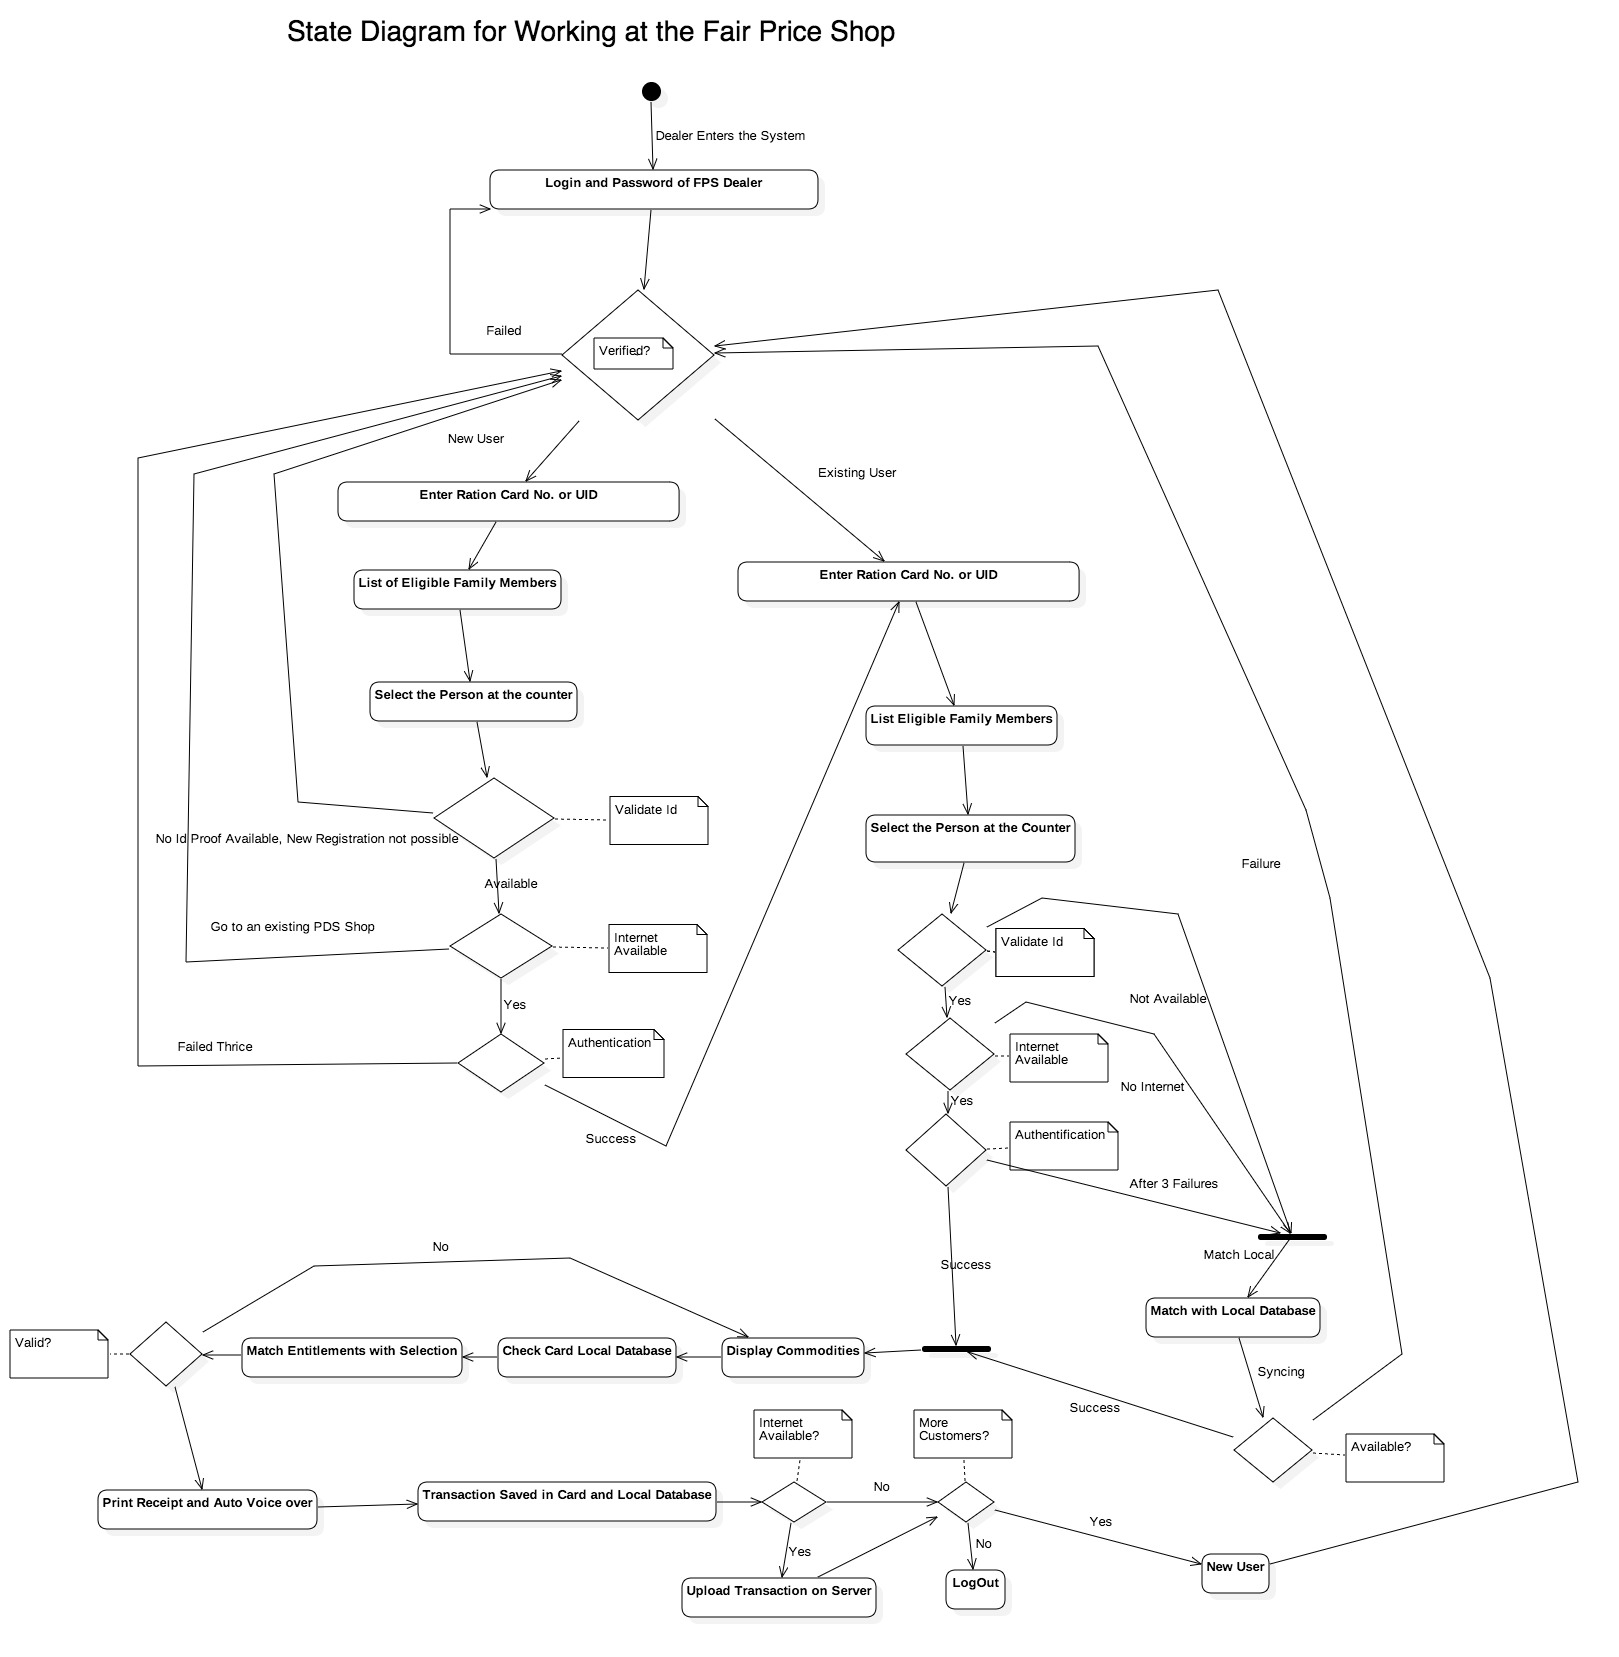
\includegraphics[width=1.1\textwidth]{FPS.jpg}
\caption{\label{fig:design}The diagram shows the various states  involved in the transaction process.}
\end{figure}

\subsection{Ration Cards}
The Ration Cards used are an amalgamation of the successes in Chhattisgarh and Tamil Nadu. We use a QR Code based Smart Card that has an inbuilt memory of the previous transactions. The memory is just like a SIM card, that can store small volumes of data. The registration of these cards is done over Fair Price Shops itself.

\subsection{Integrated Grievance Redressal Mechanism}
The user stage in Figure 2 wherein he/she has to select the grains according to entitlement will contain an integrated grievance redressal mechanism, wherein a user can press an emergency red button to notify the authorities about ill-practices at the store.
Apart from this in case the FPS shops stays closed or the user is not allowed to reach the authentication stage itself, then an active toll-free helpline exists. 
This combined with the availability of switching between FPS shops will help solve grievances of the customer.


\subsection{Transparency of Stocks}
It is essential to coalesce the transactions at FPS with technology for transparency. If the beneficiary can view the current stock status at FPS and probe into the transactions happening at FPS, the process would be more transparent. This approach will aid by 
\begin{itemize}
\item Keeping track of FPS transactions
\item Shopkeepers cannot fake and deny availability of food grains to beneficiary
\item To probe into the pattern of sales at each FPS
\end{itemize}



\subsection{SMS Alerts}
This will capture those users of the PDS who also subscribe to mobile services and not intended to be a universal implementation.
The SMS alerts give information about the arrival of grains to the Fair Price Shops and the dates when they can collect their grains.

\subsection{Modified Weighing Machines}
The problem of quantity fraud owing to uncalibrated weighing machines will be tackled by linking the weighing machine with the Point of Sale (POS) machines. Figure 3 shows the various states  involved in the calibration of weighing machines.
\begin{figure}
\centering
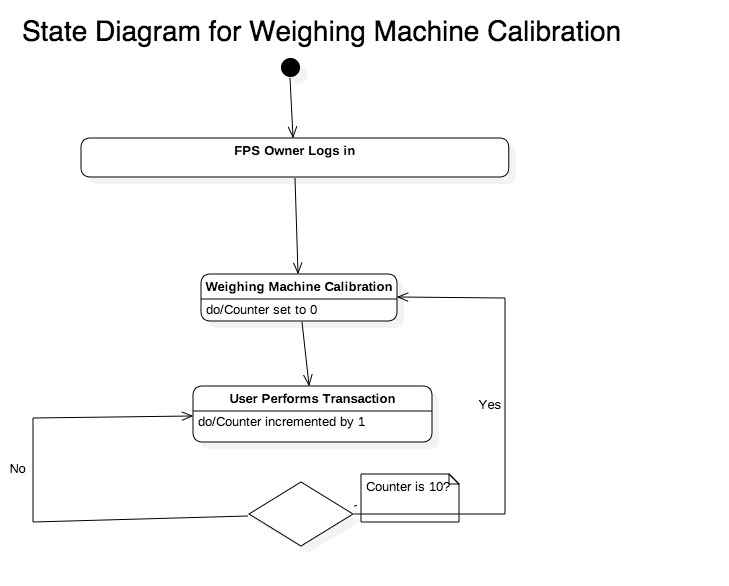
\includegraphics[width=0.7\textwidth]{Weighing_Machine.jpg}
\caption{\label{fig:wieighing}The diagram shows the various states  involved in the calibration of weighing machines.}
\end{figure}

\subsection{Fall-back mechanism for loss of card or death}
It is important to ensure that a theft or loss of card in case of the new Smart Ration Cards dispensed by us is taken into account. 
User deregistration is a very similar process to that of procuring grains. Since, this process is not about de-authenticating an identity, but of making a user de-register from a particular shop, it is much simpler and can be done at an FPS. The details are shown in Figure 4

\begin{figure}
\centering
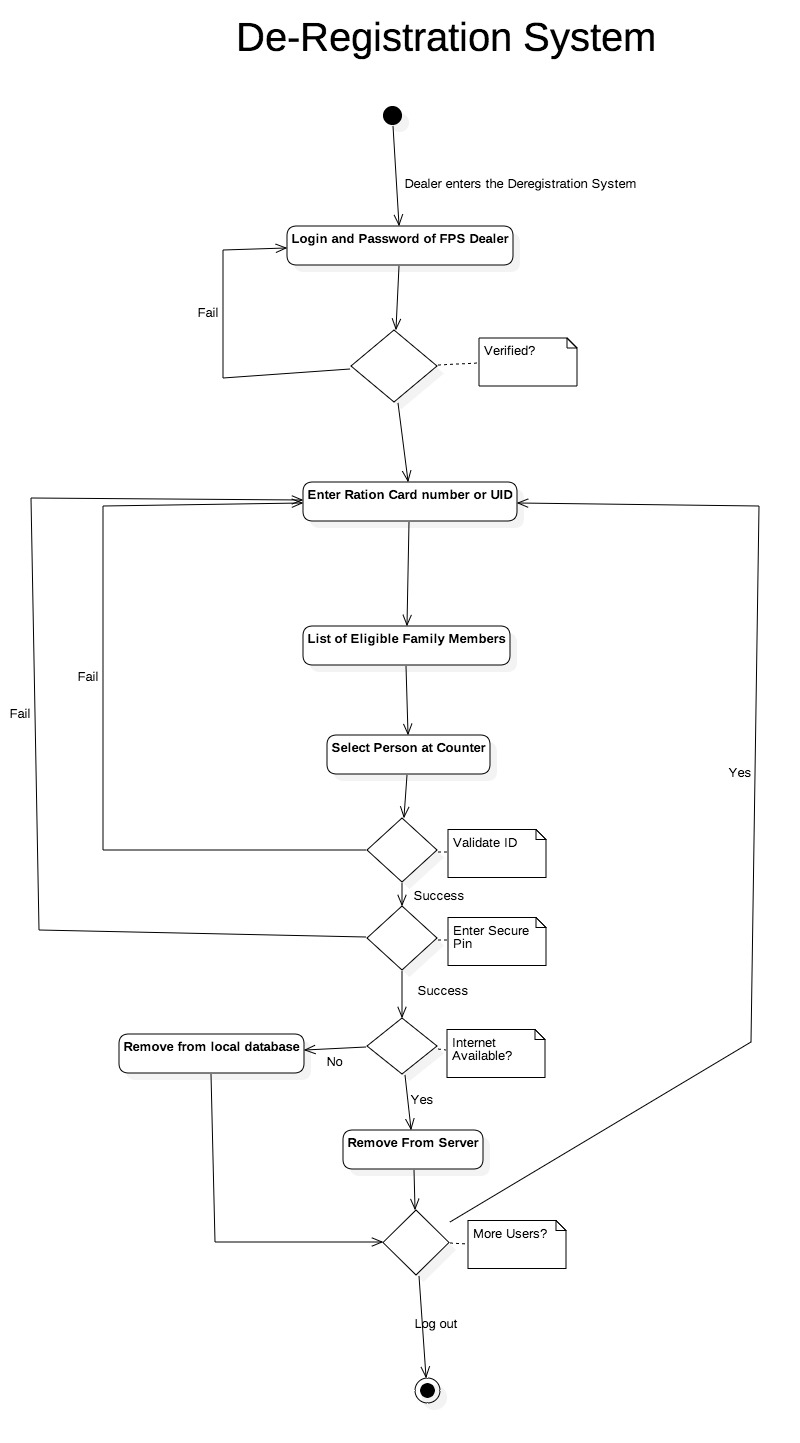
\includegraphics[width=0.7\textwidth]{dereg.jpg}
\caption{\label{fig:dereg}The diagram shows the various states  involved in user deregistration.}
\end{figure}

\section{Conclusion}

Hasty impositions of technology onto the poor can be challenging and may end up having adverse consequences. The imposition of ABBA on the PDS in Jharkhand seems to be a case of “pain without gain.” 
The system has not just led to people getting excluded from their rightful grains, but has also been an expensive experiment that has been unable to reduce quantity fraud, which is the main form of PDS corruption it was envisaged to tackle. 

The PoS system does have some helpful features. In particular, it has led to more timely and reliable recording of PDS transactions. The earlier “register” system was very defective in that respect. 

Further, the fact that ABBA prevents anyone from collecting
rations in someone else’s name is not necessarily a good
thing. For old people, being able to let a neighbour or relative
go to the ration shop on their behalf is an important facility.
In that respect, smart cards would be better than ABBA.

This paper takes a step forward into working on a \textbf{Store and Sync} design for the PDS. This design not only tackles the problem of lack of internet connectivity, but also is a gateway to eliminating the monopolistic working of FPS owners. In the present system, they have no incentive to work well, however the new model gives them a reward for working well and penalty for not.

All the changes accompanied together can indeed restore the faith of people into the PDS and help reduce the problem of distribution of grains in our country.



\section{References}
\begin{enumerate}
\item [1]  \href{http://pdsportal.nic.in/files/POS-MobileTab%20Specifications-2015-05-12-Approved.pdf}{PDS Portal : POS Mobile Tab.}
\item [2] \href{http://www.ijetae.com/files/Volume3Issue12/IJETAE_1213_69.pdf}{IJETAE Volume 3 Issue 12}
\item [3]\href{http://www.pdsportal.nic.in/Files/Final-Status_Paper.pdf}{PDS Portal: Status Paper}
\item [4]\href{http://www.pdsportal.nic.in/Files/Letter%20to%20StatesUTs%20and%20FPS%20automation%20guidelines%20dtd%2011Nov14.pdf}{PDS Portal: Automation Guidelines}
\item [5]\href{http://www.pdsportal.nic.in/Files/Implementation%20Guidelines%20Finalised.pdf}{PDS Portal: Implementation Guidelines}
\item [6]\href{https://negp.gov.in/pdfs/c6.pdf}{NEGP, Government of India}
\item [7]\href{http://www.nic.in/about-us}{National Information Centre, Government of India}
\item [8]\href{http://fcamin.nic.in/}{Consumer Affairs, Government of India}
\item [9]\href{http://planningcommission.nic.in/reports/peoreport/peo/peo_tpds.pdf} {Program Evaluation Organization, GOI, Planning Commission of India, New Delhi, March 2005  } 
\item [10]\href{http://pdscvc.nic.in/report%20on%20computersisation%20of%20PDS.htm} {Justice Wadhwa Committee Report On Computerization of PDS Operations, Delhi, February, 2009}
\item [11]\href{http://egovernance.gov.in/standardsandFramework/biometric-standards/fingerprint_image_data_standard_for_printing_Nov_10.pdf} {E-Governance: Fingerprint matching}
\item [12]\href{http://dfpd.nic.in/nfsa-act.htm}{National Food Security Act}
\item [13]COREPDS – Meri Marjee, Booklet published by Department of Food, Govt. of Chhattisgarh, 2012
\end{enumerate}


\end{document}